%%% LaTeX Template: Two column article
%%%
%%% Source: http://www.howtotex.com/
%%% Feel free to distribute this template, but please keep to referal to http://www.howtotex.com/ here.
%%% Date: February 2011

%%% Preamble
\documentclass[	DIV=calc,%
							paper=a4,%
							fontsize=12pt,%
							onecolumn]{scrartcl}	 					% KOMA-article class

\usepackage{lipsum}													% Package to create dummy text
\usepackage[brazil]{babel}										% English language/hyphenation
\usepackage[protrusion=true,expansion=true]{microtype}				% Better typography
\usepackage{amsmath,amsfonts,amsthm}					% Math packages
\usepackage[pdftex]{graphicx}									% Enable pdflatex
\usepackage[svgnames]{xcolor}									% Enabling colors by their 'svgnames'
\usepackage[hang, small,labelfont=bf,up,textfont=it,up]{caption}	% Custom captions under/above floats
\usepackage{epstopdf}												% Converts .eps to .pdf
\usepackage{subfig}													% Subfigures
\usepackage{booktabs}												% Nicer tables
\usepackage{fix-cm}													% Custom fontsizes
\usepackage[utf8]{inputenc}
\usepackage[top=2.5cm, bottom=2.5cm, left=2.5cm, right=2.5cm]{geometry}
\usepackage[ddmmyyyy]{datetime}
\usepackage{float}
\addto\captionsenglish{%
	\renewcommand\tablename{Tabela}
	\renewcommand\figurename{Figura}
} 
 

 
%%% Custom sectioning (sectsty package)
\usepackage{sectsty}													% Custom sectioning (see below)
\allsectionsfont{%															% Change font of al section commands
	\usefont{OT1}{phv}{b}{n}%										% bch-b-n: CharterBT-Bold font
	}

\sectionfont{%																% Change font of \section command
	\usefont{OT1}{phv}{b}{n}%										% bch-b-n: CharterBT-Bold font
	}



%%% Headers and footers
\usepackage{fancyhdr}												% Needed to define custom headers/footers
	\pagestyle{fancy}														% Enabling the custom headers/footers
\usepackage{lastpage}	

% Header (empty)
\lhead{}
\chead{}
\rhead{}
% Footer (you may change this to your own needs)

%% ====================================
%% ====================================
%% mude o rodape  do projeto
%% ====================================
%% ====================================

\lfoot{\footnotesize \texttt{Cabeamento estruturado} \textbullet ~Projeto - Fly Security}


\cfoot{}
\rfoot{\footnotesize página \thepage\ de \pageref{LastPage}}	% "Page 1 of 2"
\renewcommand{\headrulewidth}{0.0pt}
\renewcommand{\footrulewidth}{0.4pt}



%%% Creating an initial of the very first character of the content
\usepackage{lettrine}
\newcommand{\initial}[1]{%
     \lettrine[lines=3,lhang=0.3,nindent=0em]{
     				\color{Black}
     				{\textsf{#1}}}{}}



%%% Title, author and date metadata
\usepackage{titling}															% For custom titles

\newcommand{\HorRule}{\color{DarkGoldenrod}%			% Creating a horizontal rule
									  	\rule{\linewidth}{1pt}%
										}

\pretitle{\vspace{-30pt} \begin{flushleft} \HorRule 
				\fontsize{50}{50} \usefont{OT1}{phv}{b}{n} \color{Black} \selectfont 
				}

%% ====================================
%% ====================================
%% mude o titulo  do projeto
%% ====================================
%% ====================================

\title{Cabeamento Estruturado para escritório de consultoria}					% Title of your article goes here

%% ====================================



\posttitle{\par\end{flushleft}\vskip 0.5em}

\preauthor{\begin{flushleft}
					\large \lineskip 0.5em \usefont{OT1}{phv}{b}{sl} \color{DarkBlue}}
\author{Ansley Donizetti, Gustavo Henrique Esser}  	% Author name goes here


\postauthor{\footnotesize \usefont{OT1}{phv}{m}{sl} \color{Black} 
					\\Universidade Tecnológica Federal do Paraná - Câmpus Cornélio Procópio 								% Institution of author
					\par\end{flushleft}\HorRule}

\date{}																				% No date




%%% Begin document
\begin{document}
\maketitle
\thispagestyle{fancy} 	
\thispagestyle{empty}		% Enabling the custom headers/footers for the first page 
% The first character should be within \initial{}




%% ====================================
%% ====================================
%% mude o resumo  do projeto
%% ====================================
%% ====================================

\initial{E}\textbf{ste projeto tem como objetivo implementar uma solução de cabeamento estruturado do zero para um dos escritórios da empresa Fly Security Offensive que funciona como um centro de consultoria e treinamento, abordaremos neste projeto toda a parte de cabeamento estruturado partindo do backbone de rede ate chegar a mesa dos colaboradores da empresa. O principal objetivo é padronizar a instalação de cabos na edificação, minimizando custos e maximizando expansibilidades futuras. Este projeto contemplará o levantamento das plantas física e elaboração da planta logica da rede, e também englobaremos os custos envolvidos em equipamentos que serão implementados neste projeto. }


%% ====================================
\begin{figure}
	\centering
	
\includegraphics{utfpr}
\end{figure}

\vspace{2cm}
\centerline{\textit{\textbf{\today}}}

\clearpage
    \renewcommand*\listfigurename{Lista de figuras}
\listoffigures

\renewcommand*\listtablename{Lista de tabelas}
\listoftables


\clearpage
\renewcommand{\contentsname}{Sumário}
\tableofcontents
\clearpage

%% ====================================
%% ====================================
%% Inicio do texto
%% ====================================
%% ====================================
\section{Introdução}
Atualmente a empresa Fly Security Offensive conta com 30 colaboradores nas seguintes equipes. Administração, Comercial, Consultores, Direção e também os professores e instrutores do centro de treinamentos e consultoria em segurança da informação e redes de computadores. Com o objetivo de expandir o ramo de atuação da empresa, houve a necessidade de um escritório maior para atender melhor seus clientes e também coordenar melhor a operação da empresa.

\bigskip

Este projeto tem como objetivo, projetar e instalar uma rede de computadores no modelo LAN - \textit{(Local Area Network)} de alta capacidade no caso \textit{Gigabit Ethernet} e também disponibilizaremos todo o cabeamento para uma rede WLAN - \textit{(Wireless Local Area Network)}. Para criarmos um ambiente redundante para a empresa atualmente o escritório conta com 2 fornecedoras de link de internet fibra óptica assim mantemos a alta disponibilidade e redundância  com operadoras distintas de rede WAN - \textit{(Wire Area Network)}.

\subsection{Escopo do Projeto}
O escopo abordara o projeto e instalação de todos os componentes passivos da rede como Cabos, Tubulações, Conectores, Racks, Path Panels e demais componentes da rede que não realizam nenhum tipo de tratamento de sinais, tendo apenas a função de ser o meio físico por onde o sinal ira trafegar. Também sera elaborado o orçamento dos equipamento e mão de obra.    


\subsection{Benefícios}
Com a padronização e adequação da rede da Fly Security Offensive a empresa terá um ganho de produtividade pois toda a rede terá alta capacidade de transmissão. Outro ponto positivo com o projeto e que não teremos cabeamento telefônico pois toda a rede sera CAT 6 então conseguimos operar com telefonia VoIP sem degradar o tráfego da rede e somente em alguns casos muitos específicos necessitaremos fazer um QoS - \textit{(Quality of Service)}. Outros pontos positivos são.

\begin{itemize}
\item Facilidade de gerenciamento.
\item Maior ROI - (Retorno Sobre Investimento) para a empresa.
\item Haverá uma flexibilidade maior em todo o seu sistema. 
\item Estrtura preparada para expansões.
\end{itemize}

\subsection{Organizações Envolvidas}
O projeto sera no modelo fictício, não há nenhuma organização real envolvida. Todos os nomes das empresas são fictícias no caso meramente ilustrativa, abaixo definimos as empresas e profissionais que iram participar da implementação do projeto de cabeamento estruturado para a Fly Security Offensive.

% ---------------------------------------
% Inicio da Tabela
% ---------------------------------------

\begin{table}[h!]
	\centering
	\renewcommand{\arraystretch}{2.0}
	\caption{Empresas e profissionais envolvidos no projeto}
	\label{tab1}
	\begin{tabular}{|l|l|}
		\hline
		\multicolumn{1}{|c|}{\textbf{Empresas}} &	 \multicolumn{1}{|c|}{\textbf{Serviços e Responsabilidades}}                                 		  \\ \hline		
		Fly Security Offensive                                
		& Empresa que contratou o projeto                                              \\ \hline
		AllSafe of Networks to Cabling                             
		& Empresa responsável pelo projeto                                              \\ \hline
		Provedor de Internet Algar                                
		& Provedor de acesso à Internet                                              \\ \hline
		Provedor de Internet OI                               
		& Provedor de acesso à Internet            					\\ \hline
		Engenheiro Elétrico                                  
		& Instalações elétricas e aterramento elétrico          \\ \hline
		Telecom Local                                        
		& Instalação de linha telefônica      \\ \hline
		ANATEL                                  
		& Responsável pela certificação de redes \\ \hline
	\end{tabular}
\end{table}

% ---------------------------------------
%  Final da Tabela
% ---------------------------------------

\section{Requisitos}
Abaixo alguns requisitos do projeto que não fazem parte do espoco acordado entre ambas empresas é serão entregues pelo contrante do projeto e avaliados pelo time técnico da prestadora de serviço, assim podendo dar continuidade ao projeto de cabeamento estruturado.

\subsection{Provedor de internet - ISP}
Devera possuir no mínimo 2 links de internet contratados pela empresa, de no mínimo 1 de 200 megabytes e outro de 100 megabytes assim podendo criar uma arquitetura redundante e também confiável.  

\subsection{Estrutura predial}
A estrutura do prédio devera ter os espaços para as canaletas e tomadas de parede assim podemos trabalhar com o cabeamento horizontal e também o cabeamento backbone.  

\subsection{Rede Elétrica}
A estrutura elétrica devera ser realizada por parte da empresa contrante atendo os seguintes requisitos.
\begin{itemize}
	\item Aterramento no Backbone de rede.
	\item Nobreak com alimentação redundante.
	\item Réguas de energia no rack vindo de nobreaks diferentes.  
\end{itemize}
  	 
\subsection{Equipamentos}
Os equipamento de camada 3 no caso camada de rede deverão ser todos gigabit assim podendo garantir que todo o trafego de ponta a ponta na rede seja /1000. 

\section{Usuários e Aplicativos}
O Projeto da empresa Fly Security Offensive visa atender em torno de 30 usuários em um escritório de consultoria e treinamentos. tendo em vista que cada usuário possui um celular e também seu computador temos no minimo 60 dispositivos. Temos também a rede wireless para os clientes.
 

\subsection{Usuários}
Abaixo temos uma relação em forma de tabela todos os profissionais que atuam junto a empresa, e uma relação das aplicações que os mesmo utilizam no dia a dia de trabalho.

% ---------------------------------------
% Inicio da Tabela
% ---------------------------------------

\begin{table}[h!] % coloque h! para forcar a posicao
\centering
\caption{Modifique a legenda e crie um label}
\label{tab2} %com este label vc faz referencia no texto
\begin{tabular}{|l|l|l|l|l|}
\hline
\multicolumn{1}{|c|}{\textbf{Este é um exemplo de tabela}} & \multicolumn{2}{c|}{\textbf{C1}} & \multicolumn{2}{c|}{\textbf{C2}} \\ \hline
Você pode criar a tabela no excel                          & 1              & 2               & 3               & 4              \\ \hline
Exportar para CSV                                          & 5              & 6               & 7               & 8              \\ \hline
E importar no Table Generator                              & 9              & 10              &                 &                \\ \hline
\multicolumn{5}{|c|}{\textit{Gere o tex, e adicione em seu arquivo}}                                                             \\ \hline
\end{tabular}
\end{table}

% ---------------------------------------
%  Final da Tabela
% ---------------------------------------
\pagebreak

\subsection{Aplicativos}
Nesta seção será descrita a tabela de aplicativos e suas funções criticas no negocio. As aplicações críticas levam na frente um asterisco (*).

% ---------------------------------------
% Inicio da Tabela
% ---------------------------------------

\begin{table}[h!]
	\centering
	\renewcommand{\arraystretch}{2.0}
	\caption{Relação das aplicações da rede}
	\label{tab3}
	\begin{tabular}{|l|l|}
		\hline
		\multicolumn{1}{|c|}{\textbf{Sistema}} &	 \multicolumn{1}{|c|}{\textbf{Aplicação}}                                 		  \\ \hline
		Aplicação  *                                 
		& Sistema Interno*.
		\\ \hline	
		Internet  *                                 
		& Mecanismos de busca*.
		\\ \hline	
		Windows Server 2019 *                                 
		& AD - Active Directory*.
		\\ \hline
		Windows Server 2019 *                                 
		& File Server*.
		\\ \hline
		Windows 10                                 
		& Sistema operacional das desktop.
		\\ \hline
		Microsoft Office                                 
		& Suite de aplicações administrativas.
		\\ \hline		
	\end{tabular}
\end{table}

% ---------------------------------------
%  Final da Tabela
% ---------------------------------------

\section{Estrutura predial existente}
Conforme a planta abaixo, temos um escritório comercial de 8 cômodos não incluindo as áreas de circulação. situado no 16 andar do prédio sendo assim um duplex comercial. Conforme a planta abaixo temos também a localização dos moveis mesas, cadeiras e demais pontos de rede.  
\bigskip
Abaixo temos as áreas que serão atendidas pelo cabeamento estruturado totalizando 142.77 metros de área.
 
\begin{itemize}
	\item Recepção: 12,95 M .
	\item Sala de reunião: 13,48 M.
	\item Data Center: 3,49 M.
	\item Sala 1: 19,14 M.
	\item Comercial: 20,21 M.
	\item Suporte Técnico: 38,84 M.
	\item Coordenação: 12,46 M.
	\item Café: 6,96 M.
	\item Sala de Treinamento: 15,24 M.
	\end{itemize}

%Inicia Planta baixa tela cheia.
\clearpage 
\thispagestyle{plain}

\KOMAoptions{paper=a3, paper=landscape, DIV=20}
\recalctypearea

\begin{figure}
	%	\centering
	\noindent\makebox[\textwidth][c]{
		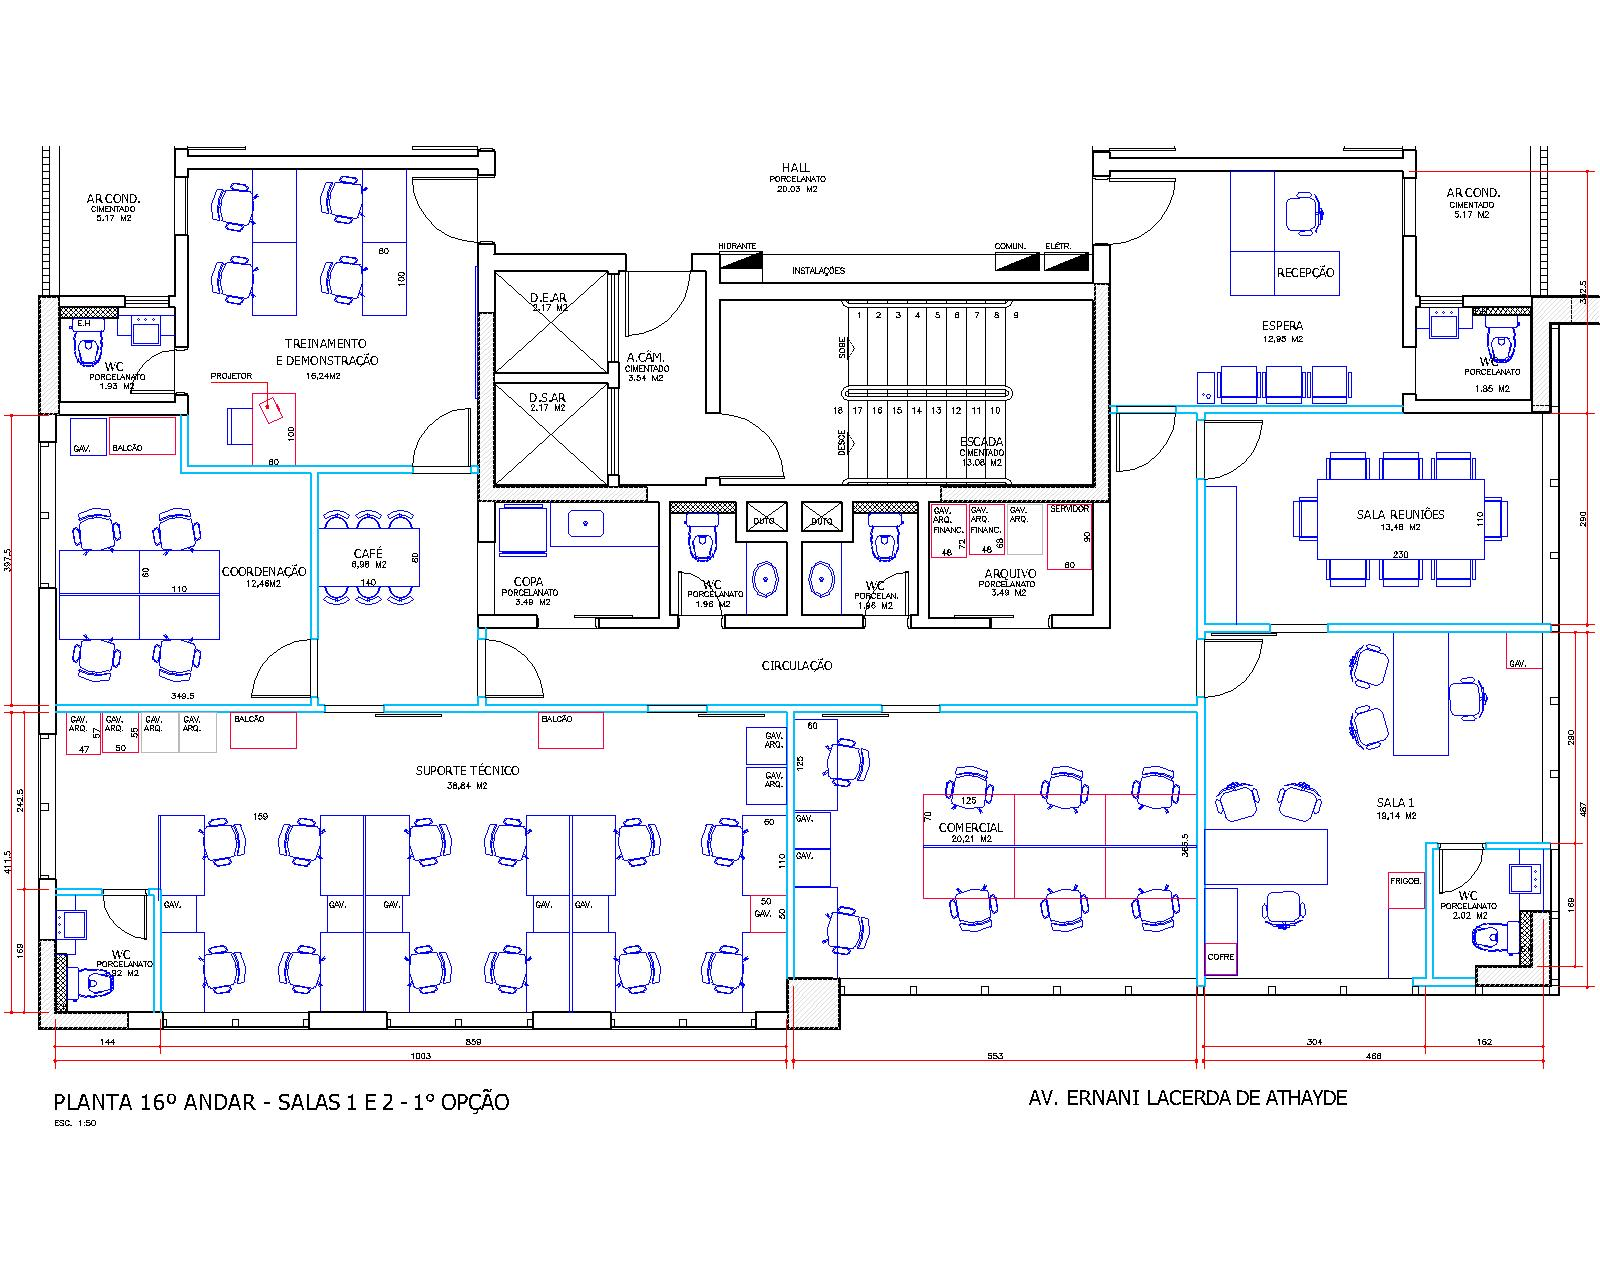
\includegraphics[width=\textwidth]{plantabaixa}
	}
	\caption{Planta Baixa - Fly Security}
	\label{plantabaixa}
\end{figure}

%Retornar ao formato A4
\clearpage
\KOMAoptions{paper=a4, paper=portrait, DIV=15}
\recalctypearea
%-- reinicio em A4

\section{Planta Lógica - Elementos estruturados}

\subsection{Cabeamento}

Conforme a figura 2 temos uma noção de como ficara os equipamentos no rack e também na figura 3 temos a  topologia física da rede.
\\

Neste projeto utilizamos a metologia Top-Down esta metodologia é estruturada, no sentido de incluir um projeto lógico de rede antes de abordar o projeto físico e abordar os requisitos antes de tudo.

A metodologia é iterativa. Novos detalhes entram progressivamente no projeto, à medida que se conhece melhor as necessidades. A Metodologia de projeto de redes Top-Down é um processo sistemático de criação de redes que tem seu foco nos aplicativos, nas metas técnicas e na finalidade dos negócios de uma organização.

\begin{figure}[H]
	%	\centering
	\noindent\makebox[\textwidth][c]{
		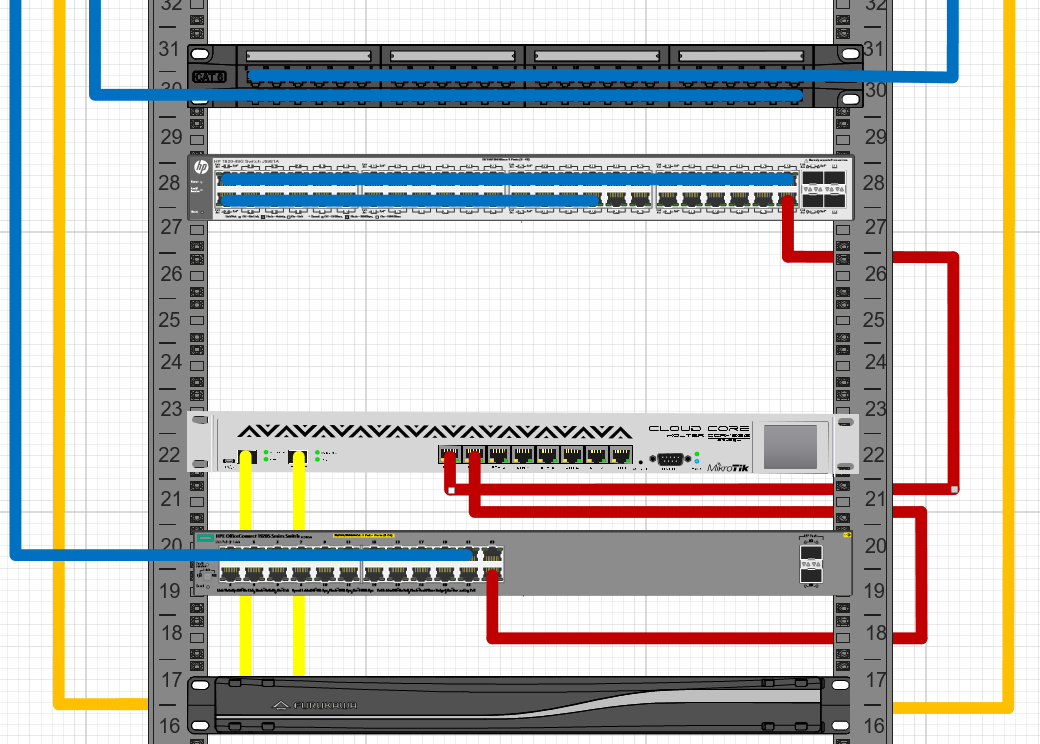
\includegraphics[width=\textwidth]{tprack}
	}
	\caption{Topologia Rack - Fly Security}
	\label{tprack}
\end{figure}

\begin{itemize}
	\item Rede Local: Azul.
	\item Rede Fibra: Amarelo. 
	\item Rede Trunk: Vermelho. 
	\item Rede WAN:   Laranja.
\end{itemize}

%Inicio Topologia Fisica tela cheia.
\clearpage 
\thispagestyle{plain}

\KOMAoptions{paper=a3, paper=landscape, DIV=20}
\recalctypearea

\begin{figure}
	%	\centering
	\noindent\makebox[\textwidth][c]{
		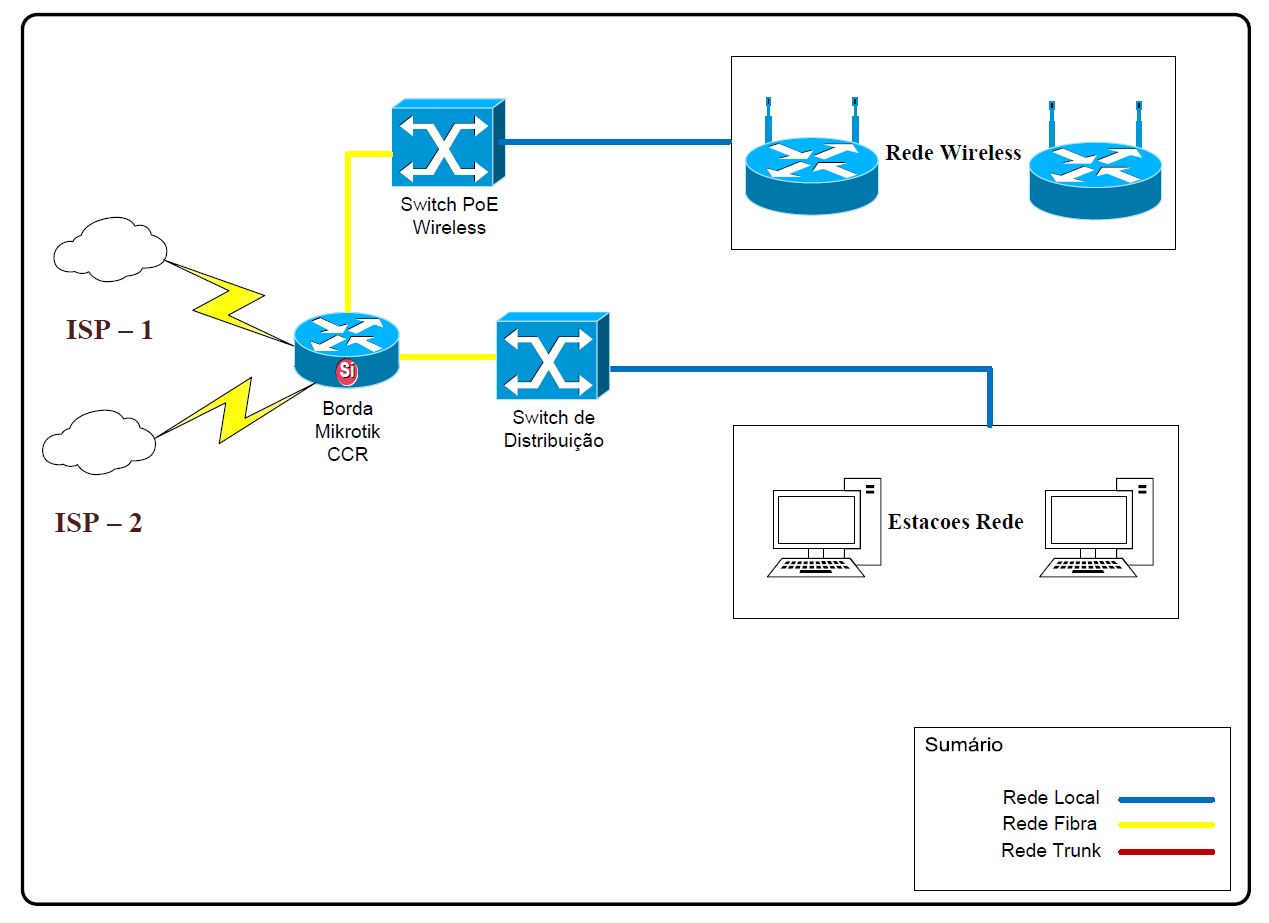
\includegraphics[width=\textwidth]{tpfisica}
	}
	\caption{Topologia Física - Fly Security}
	\label{tpfisica}
\end{figure}

%Retornar ao formato A4
\clearpage
\KOMAoptions{paper=a4, paper=portrait, DIV=15}
\recalctypearea
%-- reinicio em A4

\subsection{Topologia}

Conforme ja apresentado as topologias acima neste caso optamos por utilizar um rack fechado é um modelo mais robusto, já que é todo fechado, dificultando o acesso irrestrito e a deterioração por ação de agentes externos, como umidade, poeira etc. Além disso, o rack fechado tem a vantagem de se poder realizar o controle de circulação de ar interna, melhorando a dinâmica da temperatura dos equipamentos nele instalados — fator de extrema relevância para a operação da infraestrutura.
\\

Conforme a metologia Top-Down os dois links dos provedores - ISP chegaram em um DIO - (Distribuidor Interno Óptico) de fibra óptica assim facilitando o futuro gerenciamento da rede. 
\\

Conforme as topologias apresentas acima temos dois links de internet que chegaram no equipamento, Mikrotik CCR na porta SFP+ 1 é SFP+ 2 realizaremos a distribuição da seguinte forma.
\\

Porta ETH1 da CCR será destinada a rede cabeada da empresa que encontrasse em uma VLAN diferente da rede wireless por questões de segurança.
\\
 
Será projetado duas redes wireless uma para funcionários e uma para visitantes que terá o trafego limitado em 5Mb e será solicitado cadastro que vai ser armazenado no radius da própria CCR.
\\

Porta ETH2 da CCR será destinada ao ambiente wireless que está conectado diretamente à porta 24 do switch PoE.  

\subsection{Encaminhamento}
Neste projeto, serão instalados eletrocalhas no gesso, a eletrocalha é uma espécie de tudo metálico e rígido. Sua função é dar suporte à passagem de fios e cabos elétricos, de telefonia ou informática. Geralmente é um item que fica embutido no forro, mas sua instalação também pode ser feita de forma aparente: geralmente pendurada no teto com o auxílio de suportes.
\\

Utilizaremos eletrocalhas de PVC não o modelo metálico pois corrosão é um problema que pode levar à redução de desempenho e alteração da vida útil da instalação, pois esses materiais normalmente estão expostos à corrosão atmosférica, por isso o ambiente em que o material será utilizado é um dos principais critérios para a escolha do acabamento superficial ou do tipo de aço.

\subsection{Memorial descritivo}

		Abaixo temos em forma de tabela a relação dos equipamentos passivos que serão utilizados neste projeto, e também informaremos a quantidade de cada produto e também o fabricante recomendado.
\\

Como nosso objetivo e garantir a qualidade dos produtos e do projeto so trabalhamos com produtos da Furukawa.

% ---------------------------------------
% Inicio da Tabela
% ---------------------------------------

\begin{table}[h!]
	\caption{Equipamentos passivos}
	\label{tab8}
	\begin{center}
		\renewcommand{\arraystretch}{1.2}
		\begin{tabular}{|c|c|c|c|}
			\hline
			\textbf{Equipamento Passivo}      & \textbf{Fabricante} & \multicolumn{1}{l|}{\textbf{Quantidade}} \\ \hline
			Rack 45 U Fechado                 & Furukawa             & 1                                \\ \hline
			Patch Panel 48 Portas CAT 6      & Furukawa          & 2                                \\ \hline
			Dio  BX24 						& Furukawa  		   &
			1 								\\ \hline
			Organizador 1 U            		& Furukawa             & 2                               \\ \hline
			Cabo UTP CAT 6 450 m                 & Furukawa             & 3        \\ \hline		
			Patch Cords CAT 6 - 1,5 m (Cinza) & Furukawa                 & 35                            \\ \hline
			Patch Cords CAT 6 - 2,5 m (Vermelho) & Furukawa                 & 44                             		 \\ \hline
			Cordão Óptico 5M                     & Furukawa              & 2                                    \\ \hline
		\end{tabular}
	\end{center}
\end{table}

% ---------------------------------------
%  Final da Tabela
% ---------------------------------------


\subsection{Identificação dos cabos}
Os cabos serão identificados da seguinte forma:
\\

\textbf{ISP} = Cabos que vem do DIO e vão ate o roteador seguindo do nome do provedor.
\\

\textbf{Trunk} = Cabos que fazem a ligação do roteador ao switch.
\\

\textbf{AP} = Cabos que saem diretamente do switch PoE e vão para o AP seguido do numero do AP.
\\

\textbf{PDR} = Patch cord que liga as maquinas ao patch panel localizado no data center.
\\

\textbf{PC} = Patch cord que liga as maquinas, a tomada na parade seguido do numero do desktop.
\\


\section{Implantação}
Abaixo temos o cronograma de implantação compartilhado com o cliente. O cronograma segue os prazos estabelecidos abaixo, conforme defino com o cliente.

\begin{figure}[H]
	%	\centering
	\noindent\makebox[\textwidth][c]{
		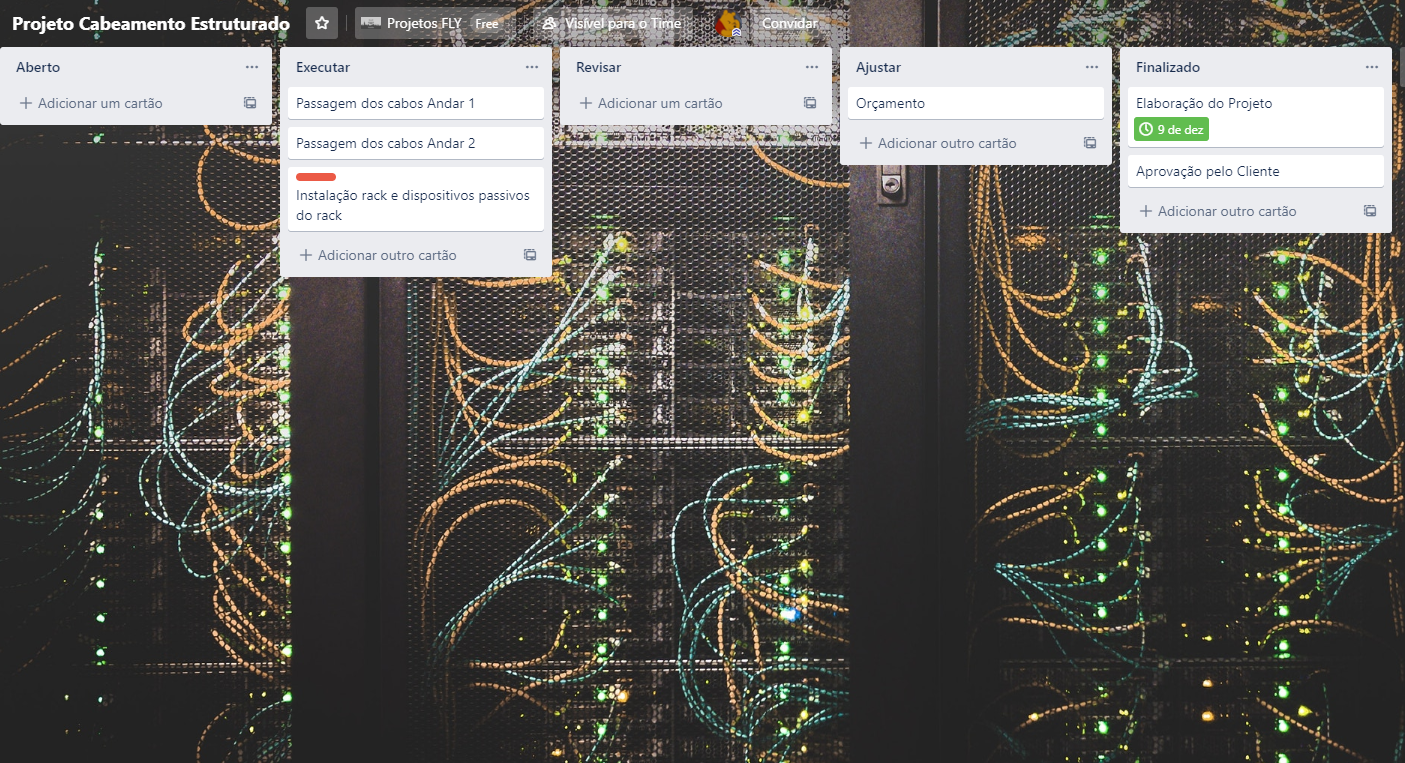
\includegraphics[width=\textwidth]{cronograma}
	}
	\caption{Cronograma Projeto - Fly Security}
	\label{tprack}
\end{figure}

\section{Plano de certificação}
A certificação da rede e infraestrutura devera ser realizada com os colaborares responsáveis pela parte técnica da empresa que acompanharam o procedimento de implantação, após o procedimento de implantação devidamente concluído e com o status operante.
\\

A participação no plano de certificação garante a entrega do resultado esperado com margem de erros aceitáveis para trabalhar em ações internas previamente realizadas antes mesmo que imprevistos ocorram de fato o que dependendo da situação poderá ocasionar problemas graves para a empresa contratante. Assim com planos de contingencia e treinamentos referente aos equipamentos instalados a margem de erro diminui drasticamente  reduzindo ainda mais os  empecilho que poderão ocorrer. 


\section{Plano de manutenção}
Caberá a equipe de TI, averiguar os status dos equipamentos se estão em pleno funcionamento, executar teste de velocidade de link de internet, testes dos equipamentos de rede. Caso alguma anomalia notada uma breve analise deverá ser realizada e informada ao nós para darmos os primeiros atendimentos e executar as providencias que devem ser tomadas.
\\

Como boas praticas, a equipe de TI, deverá gerar relatórios mensais referente ao trafego realizado internamente juntamente com os relatórios de status dos esquipamentos instalados com o objetivo de aperfeiçoarmos e otimizarmos a infraestrutura já instalada, assim prevenindo tentativas de acesso indevido de funcionários e terceiros ou até mesmo ataques externos.


\subsection{Plano de expansão}
Neste projeto de baixa complexidade, já esta considerado o esgotamento de recurso em termos de cabeamento, a necessidade de novos equipamentos como Switch e Path panel e canaletas por exemplo. Para expandir os pontos existentes, pode-se adotar a seguinte estratégia:
\begin{itemize}
	\item Patch Panel 48 Portas CAT 6.
	\item Organizador 1 U.
	\item Patch Cord CAT 6. 
	\item Cabo UTP CAT 6 450 m
\end{itemize}

\section{Risco}
O projeto demanda diretamente de um condicionamento de ar em um cômodo reservado, porem há a risco de interferência de eletromagnética.
Portanto recomenda-se de que os cabos de rede fiquem mais de 30 cm de distância da rede ou cabos que conduzem energia. A norma estabelece o mínimo de 30 cm de distância dessas linhas, pois os eletromagnetismo provindos desses cabos podem gerar ruídos na rede. Salvo desta norma cabos e conectores blindado, no entanto com a instalação dos mesmos não é apropriado devido ao custo destes cabos serem extremamente elevado, podendo tal valor ser mais compensador gastos com passagem de uma única fibra ótica e a instalação de seus conversores de mídia. A fibra ótica não captura nenhuma interferência de eletricidade. Mais detalhes referentes o cancelamento de eletro magnetismo na seção Recomendações.

\section{Orçamento}
Abaixo temos a tabela de custo dos equipamentos passivos que serão utilizados neste projeto. Não esta incluso a mão de obra neste orçamento. 

Fica estabelecido que:
\begin{itemize}
\item As partes concordam em não permitir alteração de escopo desta proposta após a sua aprovação e assinatura, ficando acordado desde já que tais mudanças, quando necessárias, acarretarão em uma nova proposta a ser elaborada pela AllSafe of Networks to Cabling, onde a mesma contemplará o novo orçamento;

\item As condições estabelecidas nesta proposta comercial são fornecidas tendo como base as informações disponibilizadas pelo cliente. Neste sentido, caso haja necessidade de alteração no projeto, para fins de adequação do mesmo ao escopo ideal, as condições ora oferecidas poderão ser revistas;

\item Valores sujeitos à alteração, sem aviso prévio, correspondentes a configuração dos equipamentos ,serviços de instalação e garantias constantes nesta proposta;

\end{itemize}
% ---------------------------------------
% Inicio da Tabela
% ---------------------------------------

  
\begin{table}[h!]
	\begin{center}
		\caption{Custo dos equipamentos passivos}
		\label{tab10}
		\renewcommand{\arraystretch}{1.2}
		\begin{tabular}{|c|c|c|c|}
			\hline
			\textbf{Equipamento Passivo}                 & \textbf{Fabricante} & \textbf{ Unitário (R\$)} & \multicolumn{1}{l|}{\textbf{Total (R\$)}} \\ \hline
			Rack 45 U Fechado                           & Furukawa             & 2.000,00                         & 2.000,00                                           \\ \hline
			Patch Panel 48 Portas CAT 6   & Furukawa            & 750,00                           & 1.500,00                                           \\ \hline
			Dio  BX24               & Furukawa             & 449,99                            & 449,99                                             \\ \hline
			Organizador 1 U           & Furukawa            & 50,00                           & 50,00                                           \\ \hline
			Cabo UTP CAT 6 450 m           & Furukawa            & 1.000,00                           & 3.000,00                                             \\ \hline
			Patch Cords CAT 6 - 1,5 m (Cinza)            & Furukawa            & 6,00                            & 210,00                                           \\ \hline
			Patch Cords CAT 6 - 2,5 m (Vermelho)            & Furukawa            & 6,00                            & 264,00                                             \\ \hline
			Cordão Óptico 5M                              & Furukawa                 & 180,00                            & 360,00                                             \\ \hline
			Conector Rj45                              & Sohoplus                 & 1,00                            & 85,00                                             \\ \hline
			\multicolumn{3}{|c|}{\textbf{Total em R\$}}                                                           & \textbf{7.918,00}                                  \\ \hline
		\end{tabular}
	\end{center}
\end{table}

% ---------------------------------------
%  Final da Tabela
% ---------------------------------------

\section{Recomendações}
Abaixo segue as observações e recomendações para o cliente.

\subsection{Cancelamento do eletromagnetismo}
Quando cargas elétricas se deslocam pelo espaço, se associam a um campo elétrico e a outro campo magnético, sendo que esses têm linhas de força perpendiculares entre si e são interdependentes. Chamamos de campo eletromagnético um fenômeno que envolve os campos elétrico e magnético variando no decorrer do tempo. É uma concentração de cargas elétricas e magnéticas que se movimentam como ondas.  Muita das vezes, especialistas técnicos em eletrônica, não possuem o conhecimento referente ao cancelamento do electromagnetismo gerado por fios de cobre. Quando colocamos cabos que possuem alta taxa de transferência de dados perto de equipamentos de energia, isso pode causar interferência e atenuações do sinal de rede prejudicando a experiencia, por isso recomendamos que os equipamentos como no-break fique com uma distancia minima de 30cm de distancia dos equipamentos de rede e caso não exista a possibilidade que seja necessário o uso de eletrocalha. Lembrando que esta interferência não influencia nos equipamentos de fibra óptica.

\subsection{Aterramento}
O “terra” é um conector que possui valor igual a zero Volt absoluto, ou seja, seu valor não se altera, diferentemente do neutro. Dessa forma, ele é o responsável por eliminar a “sujeira” elétrica dos componentes, pois toda carga eletrostática acumulada neles é descarregada para a terra. Este sistema é bem simples, consiste em uma viga cravada na terra que é conectado a um fio, geralmente da cor verde e amarela, que percorre toda a construção, com o objetivo de diminuir a variação da tensão de uma rede elétrica, eliminar as fugas de energia e proteger os usuários de um possível choque elétrico.

\subsection{Equipamentos que podem causar danos}
O estabilizador é o equipamento é responsável pela conexão de aparelhos eletrônicos a tomadas na casa dos brasileiros há décadas, antes mesmo de existirem os computadores pessoais. Isso acontece porque, desde os idos de 1940, o Brasil sofre com a instabilidade na tensão das redes elétricas, o que pode causar problemas sérios aos aparelhos eletrônicos. Promete-se aos usuários, que os dispositivos serão os principais responsáveis pelo nivelamento da tensão elétrica da rede. Com isso, picos de energia não afetariam diretamente os aparelhos. Teoricamente, sempre que a rede elétrica sobe de tensão, os estabilizadores entram em ação para regular a voltagem aplicada a cada aparelho e evitar que eles sejam queimados. Quando a rede baixa sua tensão, o processo ocorre de maneira inversa: ele é utilizado para aumentar a tensão e não deixar que os eletrônicos sejam desligados. Segundo o Departamento de Eletrotécnica da Universidade Tecnológica Federal do Paraná, tem informações que comprovam a ineficácia dos estabilizadores em redes domésticas no Brasil. Atualmente, com o desenvolvimento de fontes de alimentação universais que atuam automaticamente em redes de 127 V ou 220 V, o uso de estabilizadores é desnecessário. Estabilizadores não têm capacidade para atuar na qualidade da energia elétrica, por isso, as redes com altos níveis de poluição não têm suas tensões corrigidas, portanto não recomendados o seu uso. 

\subsection{Manutenção da energia em caso de queda}
Para equipamentos que precisem de alta disponibilidade em caso de queda de energia, o recomendado é o uso de no-break do tipo on-line de dupla conversão, que seria responsável pela entrega de senoidal. O no-break Senoidal é um equipamento de fornecimento de energia que equaliza e equilibra as ondas em seu formato mais puro (senoidal) padronizando o fornecimento de energia a fim de garantir a segurança e o funcionamento correto de aparelhos mais sensíveis como, por exemplo, aqueles utilizados na área hospitalar e médica.

\pagebreak
\section{Referências bibliográficas}

\renewcommand\refname{} %%Referências bibliográficas}  
\bibliographystyle{ieeetr}
\bibliography{referencias}    
\end{document}